%! Author = Philipp Emmenegger
%! Date = 09/06/2021

\section{Testing}
\subsection{Levels of Testing}
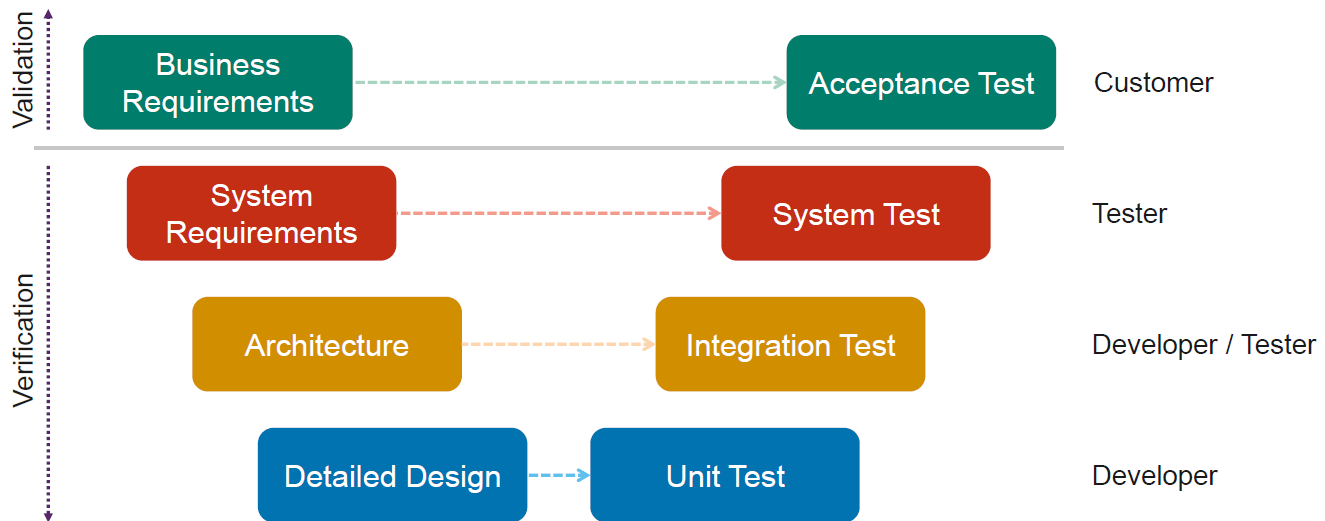
\includegraphics[width=\linewidth]{../img/levels_of_testing.png}
\textbf{Unit Tests}
\begin{itemize}
    \item Every unit is testet on its own
    \item All dependencies are broken using Test Doubles
    \item \textbf{FIRST}
    \begin{itemize}
        \item Fast
        \item Isolated
        \item Repeatable
        \item Self-Validating
        \item Timely
    \end{itemize}
    \item \textbf{AAA}
    \begin{itemize}
        \item Arrange
        \item Act
        \item Assert
    \end{itemize}
\end{itemize}
\textbf{Component Tests}
\begin{itemize}
    \item Complete components are tested
    \item Use doubles for dependencies outside of the component
\end{itemize}
\textbf{Integration Tests}
\begin{itemize}
    \item Use doubles for 'expensive' dependencies
    \item Communication between components is tested
\end{itemize}
\textbf{System Tests}
\begin{itemize}
    \item Test the full system
    \item Only use doubles if absolutely necessary
\end{itemize}

\subsection{Test Pyramid}
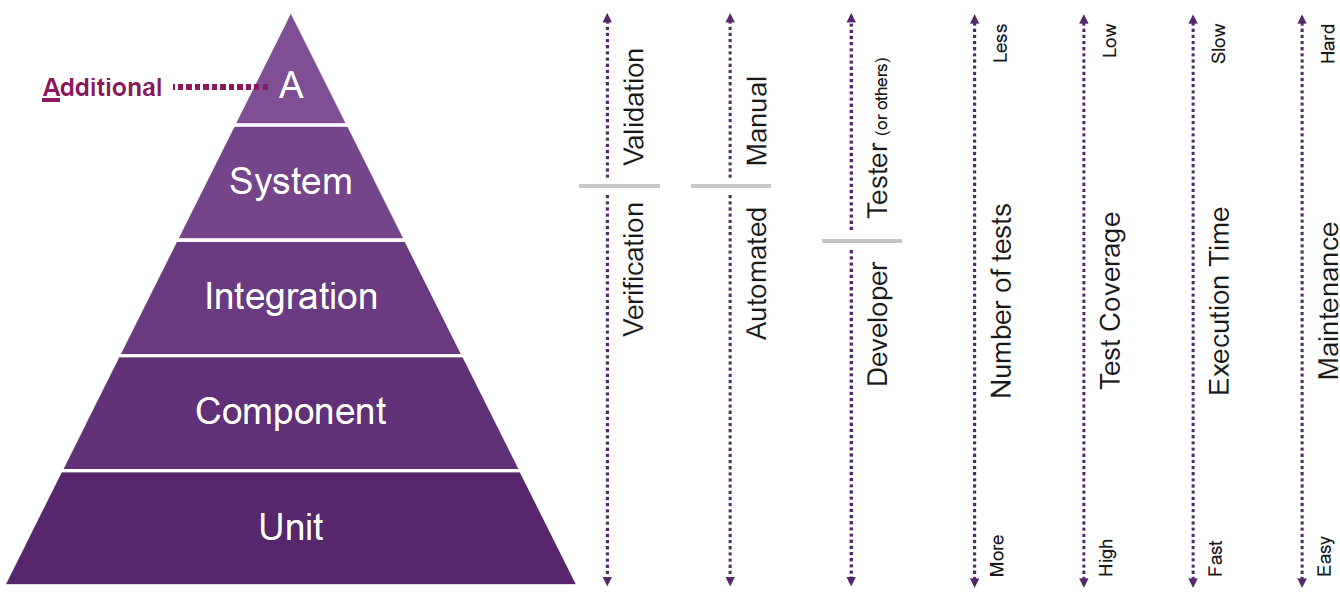
\includegraphics[width=\linewidth]{../img/test_pyramid.png}

\subsection{Environments}
\begin{itemize}
    \item DEV: Development and debugging
    \item TEST: Integration and System Tests
    \item STAGE: Acceptance Tests before releases
    \item PROD: Production
\end{itemize}
\textbf{Deployment}
\begin{itemize}
    \item DEV: On commits, pull requests, demand
    \item TEST: Every night from dev-branch
    \item STAGE: On demand before releases
    \item PROD: On demand on releases
\end{itemize}

\subsection{Integration and System Tests}
\textbf{Test Doubles}
 \begin{itemize}
     \item Pros: Faster, flexibility, less maintenance
     \item Cons: Not testing the reality (interfaces)
 \end{itemize}
\textbf{Environments}
\begin{itemize}
    \item Pros: Testing the reality
    \item Cons: Slower, less flexible, hard to maintain
\end{itemize}

\subsection{Alpha / Beta Testing}
\textbf{Alpha Testing}
\begin{itemize}
    \item Testing an early pre-release
    \item Some features might be missing
    \item Limited audience
    \item Find critical bugs before going public
\end{itemize}
\textbf{Beta Testing}
\begin{itemize}
    \item Testing the nearly finished product
    \item Feature-complete with focus on optimization
    \item Wide audience, typically external
    \item Test product within its productive environment
\end{itemize}

\subsection{Regression Testing}
\begin{itemize}
    \item Ensure that software still performs as expected after change
    \item If tests fail, that is called Regression
    \item Running unit tests after refactoring
    \item Running automated tests after a Sprint
\end{itemize}

\subsection{Performance Tests}
\begin{itemize}
    \item Manually using Integration / System tests
    \item Runtime
    \item Memory usage
    \item Power consumptions
    \item Impact of bad network quality
    \item Using Tools (Profiler)
\end{itemize}

\subsection{Monitoring}
\begin{itemize}
    \item Monitoring: Health of the system
    \item Analytics: What did the users do?
    \item Diagnostics: Where there any errors?
\end{itemize}

\subsection{A/B Testing}
\begin{itemize}
    \item User experience research methodology
    \item Compare two variants
    \item Determent which one is more effective
    \item Analytics data needed to rate efficiency
\end{itemize}

\subsection{Usability Testing}
\begin{itemize}
    \item Measure ease of use
    \item Testing product on users
    \item Observe users under controlled conditions
    \item Can be combined with A/B testing
\end{itemize}

\subsection{Paper Prototyping}
\begin{itemize}
    \item Test UI-Concepts
    \item Prototypes made from paper
    \item Helps understanding the requirements
\end{itemize}